\section{Главные циклы графа, Теорема о разложении цикла в сумму главных циклов. Применение для 
указанного графа.}

\begin{definition}
    Пусть $G (V, E)$ -- связный граф с $n$ вершинами и $r$ ребрами,
    $T (V, E_1)$ -- остовное дерево графа $G$. Ребра $e \in E_1$ называются \textit{ветвями}, ребра
    $y \in E \setminus E_1$ называются \textit{хордами} графа.
\end{definition}

Если к остовному дереву добавить хорду $y = (u,v)$, то $y$ и $T$ образуют граф с
циклом, который определяется единственным образом цепью, соединяющей
вершины $u$ и $v$. Этот цикл называют \textit{главным циклом, определяемым хордой y}.

Множество всех главных циклов называют \textit{фундаментальной системой
циклов}.

Ветвей в графе $n-1$, тогда хорд $r - (n - 1) = r - n + 1 = \mu(G)$ --
цикломатическое число графа.

\begin{definition}
    Введем операцию сложения по модулю 2 над множествами
    ребер графа $M_1$ и $M_2$:
    \begin{align*}
        M_1 \oplus M_2 = \set{e \in E | (e \in M_1 \text{ и } e \notin M_2) \text{ или } (e \notin M_1 \text{ и } e \in M_2)}.
    \end{align*}
\end{definition}
Эту операцию можно задать и для произвольного конечного числа
подмножеств ребер графа: ребро будет принадлежать сумме подмножеств
ребер, если оно принадлежит нечетному числу подмножеств.

\begin{theorem}
    Любой цикл Z графа является суммой его некоторых главных
    циклов:
    \begin{align*}
        Z = C_{i_1} \oplus \cdots \oplus C_{i_k}.
    \end{align*}
\end{theorem}

Пример. Рассмотрим граф на рисунке. Ребра остовного дерева обозначены
зеленым цветом. Построим главные циклы графа.
\begin{figure}[h]
    \centering
    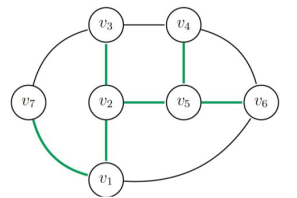
\includegraphics[scale=0.4]{29.png}
\end{figure}

Рассматриваем все хорды графа. Добавляем их по очереди в остовное дерево,
смотрим, какой цикл получился, записываем его.
\begin{align*}
    C_1 &- (v_3,v_4): v_3 \rightarrow v_4 \rightarrow v_5 \rightarrow v_2 \rightarrow v_3\\
    C_2 &- (v_4,v_6): v_4 \rightarrow v_6 \rightarrow v_5 \rightarrow v_4\\
    C_3 &- (v_1,v_6): v_1 \rightarrow v_6 \rightarrow v_5 \rightarrow v_2 \rightarrow v_1\\
    C_4 &- (v_3,v_7): v_3 \rightarrow v_2 \rightarrow v_1 \rightarrow v_7 \rightarrow v_3
\end{align*}

Получили четыре главных цикла. $C_1, C_2, C_3, C_4$ - фундаментальная система
циклов. Через нее можно выразить любой цикл.
\begin{align*}
    \text{Рассмотрим цикл } Z &= \set{v_1 \rightarrow v_2 \rightarrow v_3 \rightarrow v_4 \rightarrow v_6 \rightarrow v_1}.
    \text{ Тогда}\\
    Z &= C_1 \oplus C_2 \oplus C_3.
\end{align*}
Для того, чтобы найти разложение цикла $Z$ в сумму главных
циклов, нужно взять те циклы, которым принадлежат хорды, входящие в цикл
$Z$.